\documentclass[10pt,twocolumn,letterpaper]{article}

\usepackage{times}
\usepackage{epsfig}
\usepackage{graphicx}
\usepackage{amsmath}
\usepackage{amssymb}
\usepackage{float}
\usepackage{mathtools}
\usepackage[noend]{algorithmic}
% \usepackage{algorithm,caption}
\usepackage{amsmath}
\usepackage{algorithm2e}
\usepackage{comment}
\DeclareMathOperator*{\argmin}{arg\,min}

% Include other packages here, before hyperref.

% If you comment hyperref and then uncomment it, you should delete
% egpaper.aux before re-running latex.  (Or just hit 'q' on the first latex
% run, let it finish, and you should be clear).
\usepackage[breaklinks=true,bookmarks=false]{hyperref}


\def\cvprPaperID{****} % *** Enter the CVPR Paper ID here
\def\httilde{\mbox{\tt\raisebox{-.5ex}{\symbol{126}}}}

% Pages are numbered in submission mode, and unnumbered in camera-ready
%\ifcvprfinal\pagestyle{empty}\fi
\setcounter{page}{1}
\date{November 17, 2017}
\begin{document}

%%%%%%%%% TITLE

\title{{Progress Report CS221: Reinforcement Learning: Autonomous Race Car}}
\author{Olivier Pham\\
Stanford University\\
Management Science and Engineering\\
 {mdopham@stanford.edu}
% For a paper whose authors are all at the same institution,
% omit the following lines up until the university
% Additional authors and addresses can be added with ``\and'',
% just like the second author.
% To save space, use either the email address or home page, not both
\and
Stephanie Sanchez\\
Stanford University\\
Computational and Mathematical Engineering\\
{ ssanche2@stanford.edu}
\and
Vishal Subbiah\\
Stanford University\\
Computational and Mathematical Engineering\\
{svishal@stanford.edu}
}
\maketitle
%\thispagestyle{empty}

%%%%%%%%% ABSTRACT
%\begin{abstract}
  

%\end{abstract}

%%%%%%%%% BODY TEXT
\section{Introduction}

\subsection{Presentation of the project}

%-------------------------------------------------------------------------

Autonomous vehicles for the real world environment have been a long term ambition and in recent years endeavors towards this objective have shown very promising results. But what about autonomous driving for video games? If we can simulate autonomous driving in a game, it may give further insight to applying it in the real world. We propose to implement Reinforcement Learning (RL) to train an agent in the Open AI gym Atari game, Enduro-v0. The original goal of the game was to attain the maximum points but we decided to see if our agent could reach first place among 200 other cars. The goal is for the agent to learn from its environment and actions, the intention of the game and develop an optimal policy to win.
\begin{figure}[h]
\centering
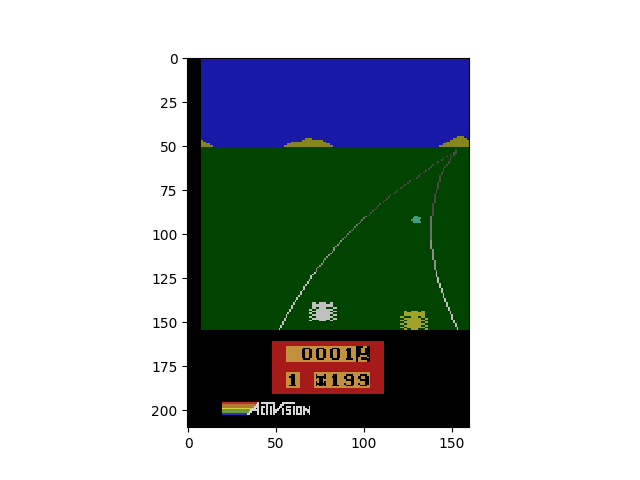
\includegraphics[width=0.8\linewidth]{img81.png}
\caption{Screenshot from the game}
\end{figure}

\begin{comment}
%-------------------------------------------------------------------------
\subsection{Related Work}

Previous work for RL and car racing used pixel values and rewards from the gym environment to learn optimal policy \cite{Car-Racing}. Other work that includes learning Atari games involves raw pixels as inputs and outputs a function that estimates future rewards that is generated by coupling of a Convolutional Neural Network (CNN) with a form of Q-Learning \cite{DeepMind}. A last take on playing Atari games defines a constant model and hyperparameter settings for the RL algorithms with a classical input features from Atari environment into the algorithms \cite{HyperParam}. \\

Some of the challenges we will face is the large state space since its a continuous game (and not turn based) and we are using the raw pixels.
\end{comment}
\subsection{Inputs and Outputs}

We will be using the OpenAI Gym environment for this project. \\
This environment provides us with pixels, rewards and a boolean indicating if the episode has ended (which happens after 13 300 frames). The observation space is a 210*160 pixels 8-bit RGB image of the screen which is represented by an array of size (210, 160, 3).\\
There are 9 possible \textbf{actions} which are:
\begin{itemize}
\itemsep-0.2em 
\item No Operation
\item Accelerate
\item Move Right
\item Move Left
\item Brake
\item Brake Right
\item Brake Left
\item Accelerate Right
\item Accelerate Left
\end{itemize}

For every state and action, the default reward is defined the following way: \[ \text{Reward(s,a,s')} = \begin{cases}1 & \text{when overtaking a car}\\-1 & \text{when crashing into another car} \\0 & \text{otherwise}\end{cases}\]


However, as the goal of the project is to learn a policy for reaching the first position as quickly as possible, we will use the following reward:
\[\text{Reward(s,a,s')} = 200 - \text{Position in the race at the state s'}\]
%We will extract the position in the race from the RGB image using a machine learning or rule based digits classifier.



%-------------------------------------------------------------------------
\subsection{Metrics}

Our first goal will be to reach the first position before the end of the game while reducing the number of cars hit. To measure our success we will assess our position at the end of the race, since we bounce backwards if we hit another car.\\

We could also explore delaying the reward to see how well the agent behaves with limited feedback. Another possible exploration is to introduce stochasticity by assigning a certain probability to the action chosen.
\\

If we manage to reach the goal and its variations, our next objective will be to reach the first position as quickly as possible. Therefore, the metric we will measure and try to minimize the number of frames required to reach the first position.



%The agent's performance will be evaluated against human performance. Aspects for assessment include: time to complete the race, racing position upon race completion, and objects hit during the race. 


%-------------------------------------------------------------------------

\subsection{Baseline and Oracle}

The Oracle for this project is to reach the first position at the end of the episode, hence its success metric is 1.\\

Our baseline is a simple approach which is to accelerate at every time step without trying to avoid other cars. After 10 games, we get an average final position of 184/200.

%-------------------------------------------------------------------------
\section{The Model}
%-------------------------------------------------------------------------
\subsection{Player Class}
The constructor for the Player class takes the Atari environment as input and utilizes an \textbf{MDP} class. The environment is used to trigger the \textbf{start state} for the player (by reseting the environment for each initialization of a player). The \textbf{actions} are as described in section 1.3 and with \textbf{probability} 1. The success and reward function is used for running Q-Learning simulation. 

We have defined a \textbf{success and probability} function that utilizes the Atari environment's step function to return a new observation based on the chosen action. The step function also returns a parameter that signals the end of the game which is our \textbf{end state}.



%-------------------------------------------------------------------------
\subsection{Reward Frame Extraction}

As OpenAI would only return 210*160 pixels an image, we needed to find a way to extract our position in the race from the screen image.
Our first approach was to extract the image of the number as an array of size 9*8 and then feed it Google Tesseract, a character recognition engine. However, the processing time was extremely slow though (approximately 1s per frame) and made running any learning learning algorithm inconceivable.\\

As digits were all the same (i.e. all the 1 are exactly alike for instance) and that there are 10 different possible characters (from 0 to 9), we figured that we needed at most 10 relevant pixels to identify the characters. This would basically make it a system of 10 variables with 10 equations.\\

Therefore, after having identified the arrays corresponding to the 10 different digits, we looked for groups of pixels which would be different on all the 10 digits array. There were no couple nor triplet of pixels which were consistently different on all the 10 arrays, but there were several quadruplets which worked. 

We chose one of them and simply mapped each combination to the corresponding number.

\begin{figure}[h]
\centering

\includegraphics[width=0.6\linewidth]{RelevantPix.png}
\caption{The four chosen pixels color values (in red) are different across all 10 digits}
\end{figure}

%-------------------------------------------------------------------------
\subsection{State Reduction}

The original RGB image returned by the environment has 210*160 pixels, which can each take a value between 0 and 255 for Red, Green and Blue. Not only did the image contain too many irrelevant information, but it also greatly increased the observation space.\\
Therefore, we decided to focus only on the important part of the screen that is to say the portion of the road in front of our vehicle, where other cars might appear. In order to reduce the observation space and hopefully decrease computation time, we reduced the quality of the image to a 4*7=28 pixels image. Finally, given that having RGB colors was not a necessity to play the game, we converted the image to greyscale, and then 3 level of black/grey/white. The final state was represented by a tuple with a length of 28.

\begin{figure}[h]
\centering

\includegraphics[width=0.6\linewidth]{81.png}
\caption{Sample image fed into our algorithm: the white pixel represents a car appearing in front of our vehicle}
\end{figure}


%-------------------------------------------------------------------------
\section{Algorithm}
\subsection{Value Iteration}
Value iteration did not perform well, since the number of frames an action runs is equally probable to be 2,3 or 4 frames. So we cannot tell the probability of each action and so value iteration only chooses a single action and does no better than the baseline.
%-------------------------------------------------------------------------
\subsection{Reduced Action Space}
To test the framework of our algorithms we reduced the action space to be: [1,7,8]. Where action 1 is accelerate, action 7 is accelerate right, and 8 is accelerate left. 

%-------------------------------------------------------------------------
\subsection{Q-Learning (exploration and learning)}
We have implemented the Q-Learning algorithm seeing how it only relies on states and actions. The implementation utilizes an explore rate, $\beta$, and a learning rate, $\alpha$ which characterizes this Q-Learning as \textbf{unsupervised learning}. \\
The algorithm follows the idea of a matrix such that each row represents a state and each column is a connected states through an action. The values of the columns are computed by the following: 

$$Q(s, a) = \alpha*(Reward(s, a) + \gamma* max(Q(s', \forall a)))$$

where $\gamma$ is the discount factor and the state inputs used are the states mentioned in section 2.3 (state reduction).\\
The idea is that we run the algorithm for a number of episodes and each episode trains the model such that the player explores its environment and collects an award until it reaches the end state. So with each episode we update/optimize our $Q(s,a)$ values. 

The updates for $\beta$ and $\alpha$ are as follows:
$$\beta = max\{\rho, min\{1, 1 - log\frac{t+1}{25}\}\}$$

$$\alpha = max\{\phi, min\{\frac{1}{2}, 1- log\frac{t+1}{25}\}\}$$

where $\rho$ = 0.01 is the min explore rate and $\phi$=0.1 is the min learning rate. \\
The explore rate governs which actions to select. If any random generated number is smaller than $\beta$ then the chosen action is randomly selected from the list of actions. Otherwise, we chose action with the max $Q(s,a)$ over all actions for the current $s$. So if the player is not exploring something new, then it will proceed with the optimal path. The results of the algorithm exhibited that the performance of the learned policy was actually worse than the random agent. The learned policy also chose to use all the actions 1,7, and 8.\\
%-------------------------------------------------------------------------

\subsection{Q-Learning (weighted)}
The weighted Q-Learning with feature extraction is as the one seen in the class homework Blackjack, but modified to fit our environment. That is, the state inputs are the rgb images returned from the environment's step function. So we approximate the Q function by the following

 $$\hat{Q}_{opt}(s,a)=w⋅*\phi(s,a) $$
 where $w$ is the weights and $\phi$ is the feature extractor function. For now the feature extractor function is the identity and all feature values are set to 1. This is one parameter that can contribute to policy results. 
 The weights are updated by
\noindent
\begingroup
  \small   
  \thinmuskip=\muexpr\thinmuskip*5/8\relax
  \medmuskip=\muexpr\medmuskip*5/8\relax  
		 $$w_{f_k} = w_{f_k} - \alpha*(Q(s,a)-(Reward(s,a)+\gamma*V_{opt}(s',a))*f_v$$
\endgroup\\
where $f_k$ is the feature key, $f_v$ is the feature value, $\alpha$ is the step size ($\frac{1}{iterations}$), and $\gamma$ is the discount. 
Like the above Q-Learning algorithm this weighted one also uses an exploration parameter to determine random based actions or the best action, however the exploration term remains constant. 
\subsection{Preliminary Results}

The exploring and learning Q algorithm was simulated with 800 iterations as seen below showing drastic fluctuation in rewards per episode.

\begin{figure}[h]
\centering
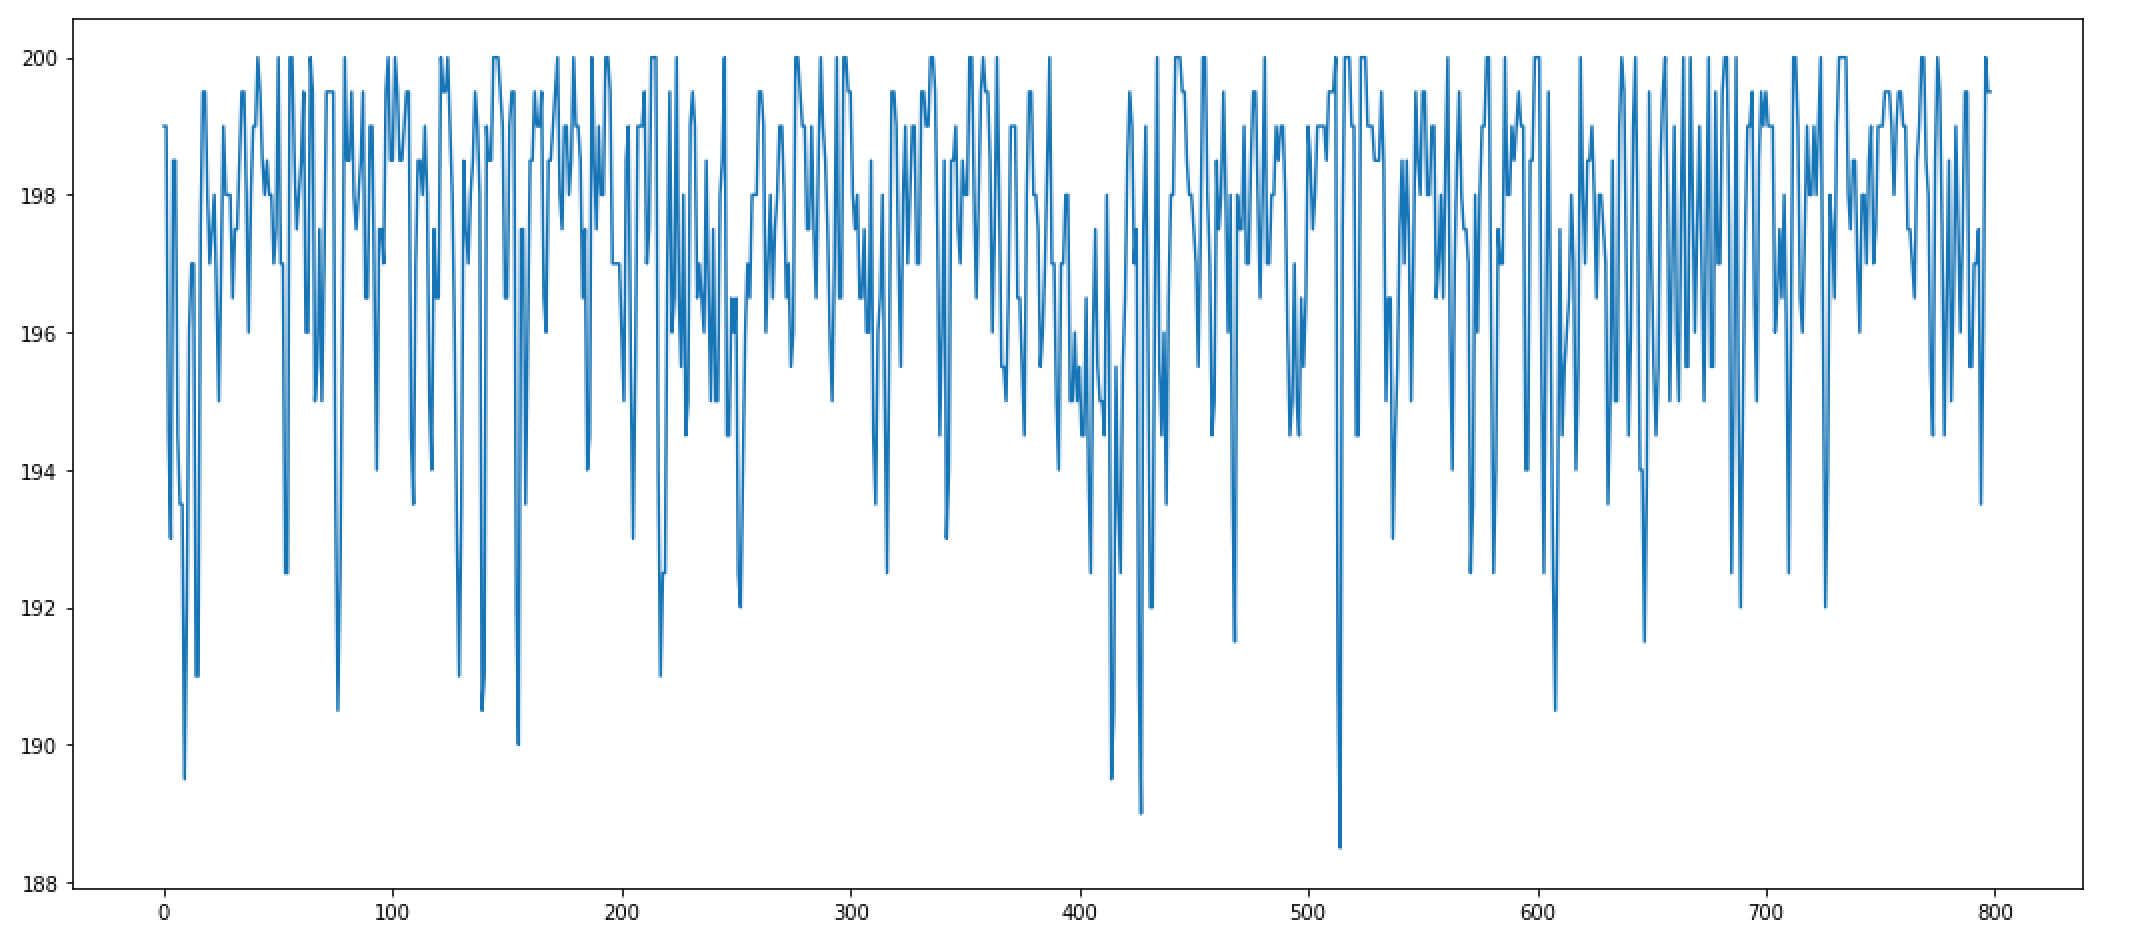
\includegraphics[width=0.6\linewidth]{qlearning_exp.png}
\caption{Plot of reward per episode with 800 iteration simulation}
\end{figure}

The weighted Q-Learning algorithm was performed by simulation for the following number of iterations: 10,20,30,40, and 50. Below are plots of the rewards returned per episode(game) in a simulation and average reward of number of iterations per simulation. It seemed that the highest rewards per episode were attained in the middle range of iterations per simulation but the average reward per simulation increased for the most part. The chosen actions for the learned policy were 8 for about half of the episode and 1 for the remainder. 
\begin{figure}[h]
\centering
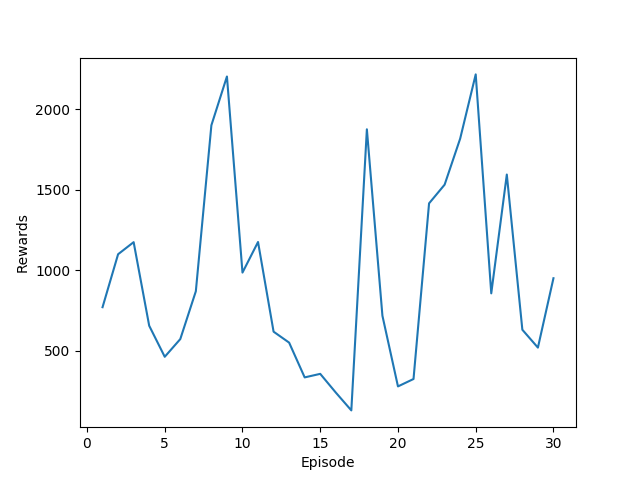
\includegraphics[width=0.6\linewidth]{numTrails_30.png}
\caption{Plot of reward per episode in a 30 iteration simulation}
\end{figure}

\begin{figure}[h]
\centering
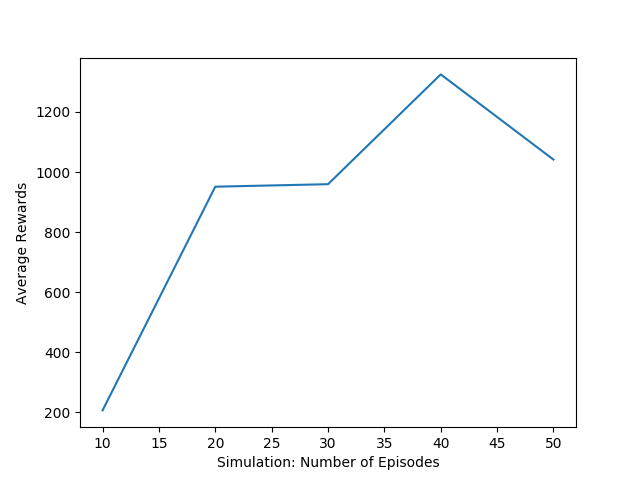
\includegraphics[width=0.6\linewidth]{avg_rewards.png}
\caption{Plot of average reward from number of iterations per simulation.}
\end{figure}


%-------------------------------------------------------------------------

\section*{Next Steps}

\subsection*{Improving the reward function}

The reward function we used so far took into account the current position of the vehicle. Hence, a bad action (for instance crashing into another car) while being in a good position is considered more valuable than a good action while being in a bad position. \\
This is probably not the best reward function as our agent doesn't properly learn to drive: some (state, action) have high q-values simply because they were visited while in a good position.\\
For the next part of our project, it would be interesting to try this reward function which doesn't implicitly take into account the current position:
\[ \text{Reward(s,a,s')} = \begin{cases}Position(s') &\\ \text{if s' if a final state}\\Position(s')-Position(s) & \\\text{otherwise} \end{cases}\]
Even in a good position, the agent will rather try to overtake some more cars.

\subsection*{Improving the state representation/features used for learning}

First, the current image fed into our algorithm might not contain enough information. It will be interesting to provide the agent with a more detailed image and let it learn through more episodes.\\
Then, the game landscape changes several times in the game, with the background turning from green to white to brown and so on, and the color of opponent vehicles change as well. Therefore, the white color which was associated with an opponent car suddenly becomes the road, which is difficult to understand for the algorithm as states no longer have the same meaning. One thing we could do to avoid this issue in the future is to normalize and standardize the color on from the greyscale screen before putting them into bin boxes: a car will be recognizable because it stands apart from the "mean color".\\
Finally, another possibility would be to manually create features out of the screen by taking specific pixels where we might go if we take a certain action, for instance the top right pixel if we plan to accelerate to the right, to see if there's a collision risk.


\subsection*{Algorithms}
The Q-learning algorithms we have implemented so far store the best action for a given state as a table and its corresponding Q value. We could proceed with implementing a neural network, where it approximates the Q value function. This would lead to developing a deep Q-learning Network. Deep Q-learning networks usually allow us to explore more complex states and so we may not need to reduce the state space or action space, and directly use the raw pixel information. We would build a convolutional neural network like a VGGNet or of similar architecture.  

We could also try implementing Monte Carlo Search Tree using compulsive deliberation to compare how a general game playing algorithm does compared to reinforcement learning 


\begin{thebibliography}{9}
\bibitem{Car-Racing} 
M. A. Farhan Khan, Oguz H. Elibol
\textit{Car Racing using Reinforcement Learning}. 

 
\bibitem{DeepMind} 
Volodymyr Mnih, Koray Kavukcuoglu, David Silver, Alex Graves, Ioannis Antonoglou,
Daan Wierstra, Martin Riedmiller
\textit{Playing Atari with Deep Reinforcement Learning}. 


\bibitem{HyperParam} 
David Hershey, Rush Moody, Blake Wulfe
\textit{Learning to Play Atari Games}. 

\end{thebibliography}
\end{document}
